\section{Nodal integration}


In weak form methods it turns out that normal integration schemes do not retain the conservation properties of the IMR.
The problem is that (outside of the infinite node limit) weak form equations make statements about the integral properties of the solution, whereas magnetisation length is a nodal property.
The solution is to use a non-typical quadrature scheme which directly links the nodal values with the integral values.
The downside of such schemes is that the accuracy of the evaluation of integrals is reduced.

In the micromagnetics literature this is known as reduced integration\cite{Cimrak2008}.
However in other finite element literature ``reduced integration'' refers to using lower order Gaussian quadrature than needed to exactly integrate the shape and test functions.
The term ``Nodal integration'' is more the standard term for schemes where the nodal values are used directly in the quadrature (typically with mesh-free methods \eg \cite{Puso2008}).

In this section we first show why standard quadrature schemes cannot have the required conservation properties.
We then show that the introduction of nodal integration schemes reattains the conservation properties.
Finally we present some numerical experiments.



\subsection{Failure of $\abs{\mv}$ conservation with Gaussian quadrature}

\newcommand{\ipg}[2]{\intd{{#1} \cdot {#2}}}

We begin with the weak form of the LLG equation
\begin{equation}
  \label{eq:weak-llg}
  \intd{\dmdt \cdot \testv + \mv \times \hv[t, \mv] \cdot \testv - \dampc \mv \times \dmdt \cdot \testv} = 0, \quad \forall \testv
\end{equation}
where $\testv = \threevec{\test}{\test}{\test}$ and $\test \in \ts$ is a scalar test function.

\newcommand{\midpoint}[1]{\hat{#1}}
\newsubcommand{\mvm}{\midpoint{\mv}}{n}
\newcommand{\tm}{\midpoint{t}_n}

\newcommand{\pdsub}[3]{\mathrlap{\pd{#1\mathrlap{_{#2}}}{#3}}\phantom{\pd{#1_{#2}}{#3}}}
\newcommand{\dtop}{\delta}
\newcommand{\dmdtm}{\pdsub{\mv}{n}{t}}
\newcommand{\dmdtml}{\pdsub{\mv}{n,l}{t}}
\newcommand{\dmdtmj}{\pdsub{\mv}{n,j}{t}}

% To simplify the notation we use inner product notation for the integral of a dot product:
% \begin{equation}
%   \intd{\av \cdot \bv} = \ipg{\av}{\bv}.
% \end{equation}

Substituting in the IMR we obtain
\begin{equation}
  \label{eq:weak-llg-imr}
  \ipg{\dmdtm}{\testv} + \ipg{(\mvm \times \hv[\tm, \mvm])}{\testv} - \dampc \ipg{(\mvm \times \dmdtm)}{\testv} = 0, \quad \forall \testv .
\end{equation}

where $\midpoint{x} = \frac{x_{n+1} + x_{n}}{2}$ is the midpoint value of $x$ and $\dtop x = \frac{x_{n+1} - x_n}{\dtn}$ is the midpoint derivative.

To obtain our result we examine the case where $\testv = \mvm$.
Note that $\mvm$ is in the vector space of test functions because we are using identical test and shape function spaces and $\mvm$ at any point must only be a linear combination of shape functions.
So by \eqref{eq:weak-llg-imr}, and using the fact that $(\av \times \bv) \cdot \av) = 0$ we have
\begin{equation}
\label{eq:23}
  \begin{aligned}
    0 &= \ipg{\dmdtm}{\mvm}, \\
    &= \frac{1}{2\dtn} \intd{(\mv_{n+1} + \mv_{n}) \cdot (\mv_{n+1} - \mv_n)}, \\
    &= \frac{1}{2\dtn} \intd{\abs{\mv_{n+1}}^2 - \abs{\mv_{n}}^2}.
  \end{aligned}
\end{equation}

At first glance it appears that we have achieved conservation. However this is only an integral relationship, meaning that the values of the integrand at the nodes are not constrained.
We can see this in more detail by substituting in the space interpolation of $\mv$ at the Gaussian integral evaluation points.
Dropping the constant factor of $2\dtn$ and assuming that $\abs{\mv_n} = 1$ everywhere this gives
\begin{equation}
  \begin{aligned} 
    1 &= \intd{\abs{\sum_k \mv_{n+1, k} \tbf_k(\xv)}^2}, \\
    &= \sum_l w_l \abs{\sum_k \mv_{n+1, k} \tbf_k(\xv_l)}^2.
  \end{aligned} 
\end{equation}

This can be satisfied without requiring that all $\abs{\mv_{n+1, k}} = 1$.
For example if we set the number of nodes to two (a 1D problem with linear shape functions) and assume magnetisation only along the $z$-axis then this condition becomes:
\begin{equation}
  \begin{aligned}
    1 &= \sum_l w_l \abs{\sum_k \mv_{n+1, k} \tbf_k(\xv_l)}^2, \\
    &= w_0 (m_0 a + m_1 b)(m_0 a + m_1 b) + w_1 (m_0 c + m_1 d)(m_0 c + m_1 d), \\
    &= m_0^2 (w_0 a^2 + w_1 c^2) + m_1^2 (w_0 b^2 + w_1 c^2) + m_0 m_1 (2w_0ab + 2w_1cd), \\
    &= m_0^2 \alpha + m_1^2 \beta + m_0 m_1 \gamma, \\
  \end{aligned}
\end{equation}
where $a,b,c,d$ are the values of shape functions at the integration points, $m_l = m_{z}$ at node l and $\alpha, \beta, \gamma$ are constants.
So given any $m_{z,0}$ we can solve the above expression to find an $m_{z,1}$ that satisfies the constraint.
Since $m_z$ all magnetisation is along the $z$-axis in this example we can vary magnetisation length arbitrarily while still satisfying the constraint.

A similar expression is obtained if nodal magnetistations are chosen for the test function used in \eqref{eq:23} instead of the magnetisation function, as in \autoref{sec:weak-cons-absmv}.

Finally it is interesting to note that if the magnetisation is constant in space at times $t_n$ and $t_{n+1}$ then the integral condition in \eqref{eq:23} \emph{is} sufficient to give conservation of the magnetisation length at nodes.


\subsection{Failure of energy conservation with Gaussian quadrature}

The proof of energy conservation does not fail directly.
However, non-constant magnetisation length means that the derivation of the boundary condition is no longer applicable (??ds check this, non-constant |m| should destroy Neumann condition therefore symmetry is gone).
Hence the effective field is no longer symmetrical and the proof of energy conservation no longer applies.

\subsection{A nodal integration scheme}

In order to regain conservation properties in a weak-form-based method we introduce a nodal integration scheme based on that used by Bartels et. al.\cite{Bartels2006}:
\begin{equation}
  \label{eq:nodal-integration}
  \int f(\xv) \d \xv \approx \sum_{l\in \text{nodes}} \beta_l f(\xv_l),
\end{equation}
where $\beta_l$ is a weight.
This is simply the weighted sum of the value of the integrand at nodes.

As an additional benefit this greatly simplifies the calculations since no interpolation of the values to the integration points is needed.
For example with reduced integration (and using that $\tbf_k(\xv_l) = \delta_{kl}$) the residual contribution of the time derivative term of LLG of test function $k$ becomes
\begin{equation}
  \begin{aligned}
    \intd{\dmdt \cdot \tbfv_k} &= \frac{1}{\dtn} \intd{(\mv_{n+1}(\xv) + \mv_{n}(\xv)) \cdot \tbfv_k(\xv)}, \\
    & = \frac{1}{\dtn} \sum_{l\in \text{nodes}} \beta_l (\mv_{n+1, l} + \mv_{n, l}) \cdot \tbfv_k(\xv_l), \\
    & = \frac{1}{\dtn} \beta_k (\mv_{n+1, k} + \mv_{n, k}) \cdot \threevec{1}{1}{1}.
  \end{aligned}
\end{equation}

% \subsubsection{Derivation of weights for local integration}

We now need to derive a suitable $\beta_l$.
To do so we represent the quadrature scheme as an integral of an interpolating polynomial which matches the desired integration scheme, then we rearrange the equation to find the weights (see, \eg \cite[480]{Kincaid2002}).
In \texttt{oomph-lib} all integration is done in local co-ordinates (as discussed in \autoref{sec:fem-integration-??ds}), so we now calculate weights applicable in this case.

A suitable quadrature-interpolation-polynomial for our case is the shape/test function for the node.
So we have:
\begin{equation}
\label{eq:nodal-quad-weights}
  \begin{aligned}
    \int_{\magd_e} f(\xv) \d \xv &= \int_{\magd_e} f(\sv) \pd{\sv}{\xv} \d \sv, \\
    &\approx \int_{\magd_e} \sum_l f(\sv_l) \tbf_l(\sv) J_l \d \sv, \\
    &\approx  \sum_l f(\sv_l) J_l \int_{\magd_e} \tbf_l(\sv)  \d \sv,
  \end{aligned} 
\end{equation}
where $J_l =  \evalat{\pd{\sv}{\xv}}_{\sv=\sv_l}$ is the Jacobian of the transformation from local to global coordinates evaluated at the $l$-th integration point.
Comparing \eqref{eq:nodal-integration} with \eqref{eq:nodal-quad-weights} we see that
\begin{equation}
  \beta_l =  \int_{\magd_e} \tbf_l(\sv)  \d \sv.
\end{equation}
The equivalent weight for global integration is $\beta_l = \int_{\magd} \tbf_l(\xv) \d \xv$, as used by Bartels \etal\cite{Bartels2006}.

If $f(\sv)$ is a linear polynomial then our nodal quadrature scheme is exact.
However most terms in the LLG residual are higher order, due to them containing one or more interpolated terms (each a linear polynomial) mulitiplied by a test function (also a linear polynomial).
An exception is the exchange residual, \eg the $x$-component:
\begin{equation}
  \begin{aligned}
    \rex_{,x} = - \intd{ m_y \bigb{\grad \tbf \cdot \grad m_z}} + \intd{ m_z \bigb{\grad \tbf_n \cdot \grad m_y}},
  \end{aligned}
\end{equation}
which is linear because the gradient terms are constants ($m_i$ and $\tbf_n$ are linear polynomials so their derivatives are constant).
Hence the exchange term is integrated exactly.



\subsection{Conservation of $\abs{\mv}$ at nodes}
\label{sec:weak-cons-absmv}

Starting from the IMR discretised weak form of the LLG \eqref{eq:weak-llg-imr}:
\begin{equation}
  \intd{\dmdtm \cdot \testv + (\mvm \times \hv[\tm, \mvm]) \cdot \testv - \dampc (\mvm \times \dmdtm) \cdot \testv }= 0, \quad \forall \testv .
\end{equation}

We examine the choice of the test function as the midpoint nodal value of $\mv$ at node j multiplied by the $j$th test basis function, $\testv = \mvm_{,j} \tbf_j$.
This choice is clearly in the vector space of test functions because it is simply a constant multiple of a basis function.
The resulting 
\begin{equation}
  \sum_l \beta_l \bigs{\dmdtml \cdot \mvm_{,j}\tbf_j(\xv_l) + (\mvm_{,l} \times \hv[\tm, \mvm_{,l}]) \cdot \mvm_{,j}\tbf_j(\xv_l) - \dampc (\mvm_{,l} \times \dmdtml) \cdot \mvm_{,j}\tbf_j(\xv_l)} = 0.
\end{equation}

Using $\tbf_k(\xv_l) = \delta_{kl}$ we can eliminate the summation
\begin{equation}
  \beta_j \bigs{\dmdtmj \cdot \mvm_{,j} + (\mvm_{,j} \times \hv[\tm, \mvm_{,j}]) \cdot \mvm_{,j} - \dampc (\mvm_{,j} \times \dmdtmj) \cdot \mvm_{,j}} = 0.
\end{equation}
By the properties of the triple product the procession and damping terms vanish. Then expanding the midpoint values gives us our conservation result:
\begin{equation}
  \begin{aligned}
    \frac{\beta_l}{2\dtn}(\mv_{n+1,j} - \mv_{n,j}) \cdot (\mv_{n+1, j} + \mv_{n, j}) &= 0, \\
    \abs{\mv_{n+1, j}}^2 - \abs{\mv_{n, j}}^2 &= 0.
  \end{aligned}
\end{equation}

This can obviously be repeated for all nodes $j$, hence each nodal magnetisation length is conserved.


\subsection{Energy loss}

Again we start from the IMR discretised weak form of the LLG \eqref{eq:weak-llg-imr} and proceed by choosing specific test functions.
In this case we first choose $\testv = \dmdtm$, which gives:
\begin{equation}
  \label{eq:test-dmdt}
  \begin{aligned}
    0 &= \intd{\dmdtm \cdot \dmdtm} - \intd{\dmdtm  \cdot (\mvm \times \hv[\tm, \mvm])}.
  \end{aligned}
\end{equation}

Secondly we choose $\testv = \hv[\tm, \mvm]$ to obtain:
\begin{equation}
  \label{eq:test-h}
  \begin{aligned}
    0 &= \intd{\dmdtm \cdot \hv[\tm, \mvm]} - \dampc \intd{\hv[\tm, \mvm] \cdot (\mvm \times \dmdtm)}, \\
    & = \intd{\dmdtm \cdot \hv[\tm, \mvm]} - \dampc \intd{\dmdtm \cdot (\hv[\tm, \mvm] \times \mvm)}, \\
    & = \intd{\dmdtm \cdot \hv[\tm, \mvm]} + \dampc \intd{\dmdtm \cdot (\mvm \times \hv[\tm, \mvm])}.
  \end{aligned}
\end{equation}

Combining equations~\eqref{eq:test-dmdt} and \eqref{eq:test-dmdt} results in
\begin{equation}
  0 = \intd{\dmdtm \cdot \hv[\tm, \mvm]} + \dampc \intd{\dmdtm \cdot \dmdtm},
\end{equation}
\ie
\begin{equation}
  \intd{\mv_{n+1} \cdot \hv[\tm, \mvm]} = \intd{\mv_n \cdot \hv[\tm, \mvm]} - \dtn \dampc \intd{\dmdtm \cdot \dmdtm}.
\end{equation}
With zero applied field $\hv[t, \mv] = \hv[\mv]$ is a symmetrical linear operator on $\mv$ with respect to the inner product $\intd{\av \cdot \bv}$ (see \autoref{sec:energy-field-relation}), using this property in a similar manner to \autoref{sec:prop-imr-llg} we obtain
\begin{equation}
  \frac{1}{2}\intd{\mv_{n+1} \cdot \hv[\mv_{n+1}]} = \frac{1}{2}\intd{\mv_n \cdot \hv[\mv_n]} - \dtn \dampc \intd{\dmdtm \cdot \dmdtm}.
\end{equation}
But, as mentioned in \autoref{sec:prop-imr-llg} $\frac{1}{2}\intd{\mv \cdot \hv[\mv]}$ is the total micromagnetic energy of the domain (when $\happ = \zerov$), hence we have
\begin{equation}
  \e_{n+1} = \e_n - \dtn \dampc \intd{\dmdtm \cdot \dmdtm},
\end{equation}
which is the midpoint discretisation of the analytical energy loss rate given by equation~\eqref{eq:energy-decay}.
In particular when $\dampc = 0$ the energy is conserved.

The extension to the case with the applied field proceeds exactly as for the strong form of the LLG, as discussed in \autoref{sec:prop-imr-llg}.
The final result is
\begin{equation}
  ??ds
\end{equation}


\subsection{Numerical experiments}
\label{sec:numer-exper}

In the following experiments we use the wave exact solution in 2D (see \autoref{sec:wave-like-solution}) for simplicity and because an exact solution is known.
The solution parameters used are $\kvec = 2\pi$ so that the solution is periodic on domains of unit size and $c = 0.35\pi$ which gives large amplitude oscillations without while still remaining in the wave-like parameter regime.

The Newton tolerance is set to $10^{-14}$ unless otherwise specified.
The linear systems are solved using GMRES with an ILU-1 preconditioner.


\subsubsection{Accuracy of nodal quadrature}



\subsubsection{Convergence}

Since we have an exact solution for this example we can calculate the total error and plot the convergence as $\dtn \goesto 0$ and $h \goesto 0$.
Following the example of Jeong \etal\cite{Jeong2014} we link the spatial discretisation length to the time step by $\dtn = 0.32h$.

We plot two figures: convergence of a single step and convergence after some time.

??ds


\subsubsection{Magnetisation length conservation}

First we examine the evolution of the magnetisation length error over time in a single case.
We used $\dampc = 0.001$, a mesh of square elements with $6561$ nodes and constant time step sizes of $\dtn = 0.001$. 
These choices of mesh and time step resolve the solution well, as can be seen in the convergence experiments above.
The maximum time was $t_{max} = 5$ ($\approx 20$ wave periods), the damping is small enough that the oscillations continue well past this time. % trace in folder ??ds check it
\autoref{fig:mean-ml-error-2d-gauss} shows the behaviour of the maximum (over all nodes) error in magnetisation length, \autoref{fig:mean-ml-error-2d-nodal} shows the equivalent plot when using nodal quadrature.
When using nodal quadrature the error never grows much larger than the Newton tolerance, whereas when using Gaussian quadrature the error grows to $\order{10^{-5}}$ within the short simultation.

\begin{figure}[ht!]
  \centering
  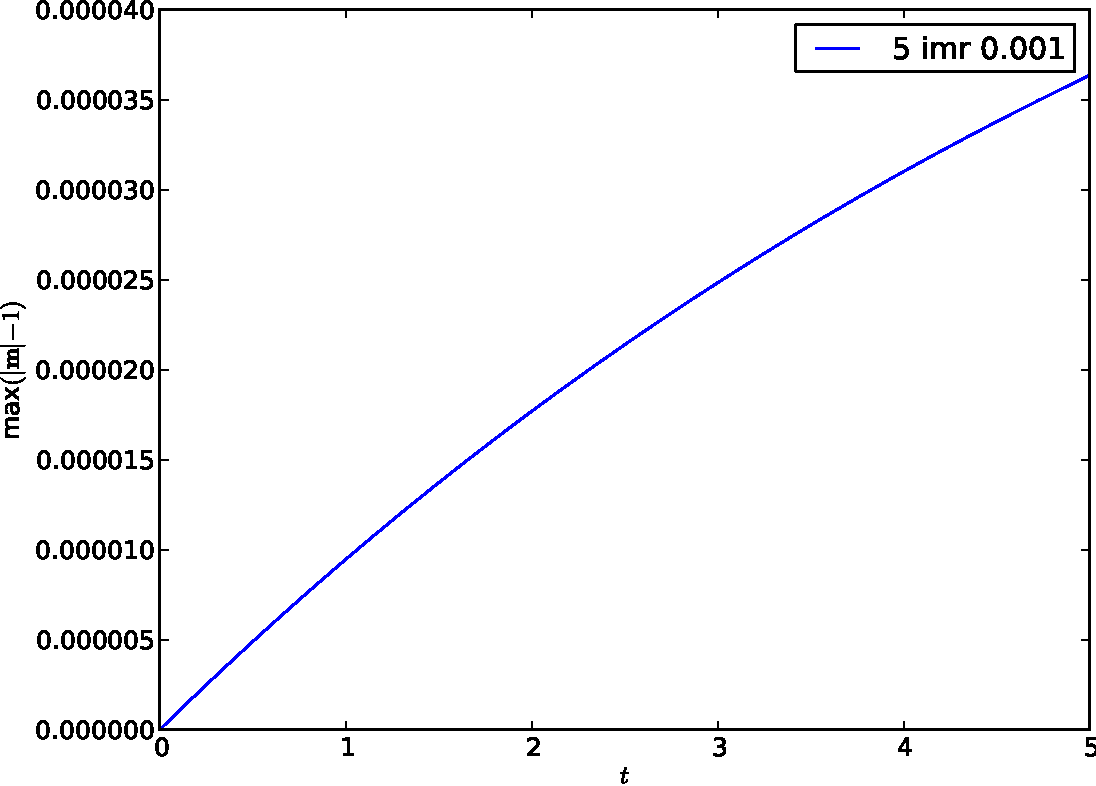
\includegraphics[width=0.8\textwidth]{plots/2d_wave_solution_m_length/gauss-maxmathbfm-1vst.pdf}
  \caption{Evolution of the maximum error of nodal magnetisation lengths in the 2D wave example with a standard Gaussian quadrature scheme.}
  \label{fig:mean-ml-error-2d-gauss}
\end{figure}

\begin{figure}[ht!]
  \centering
  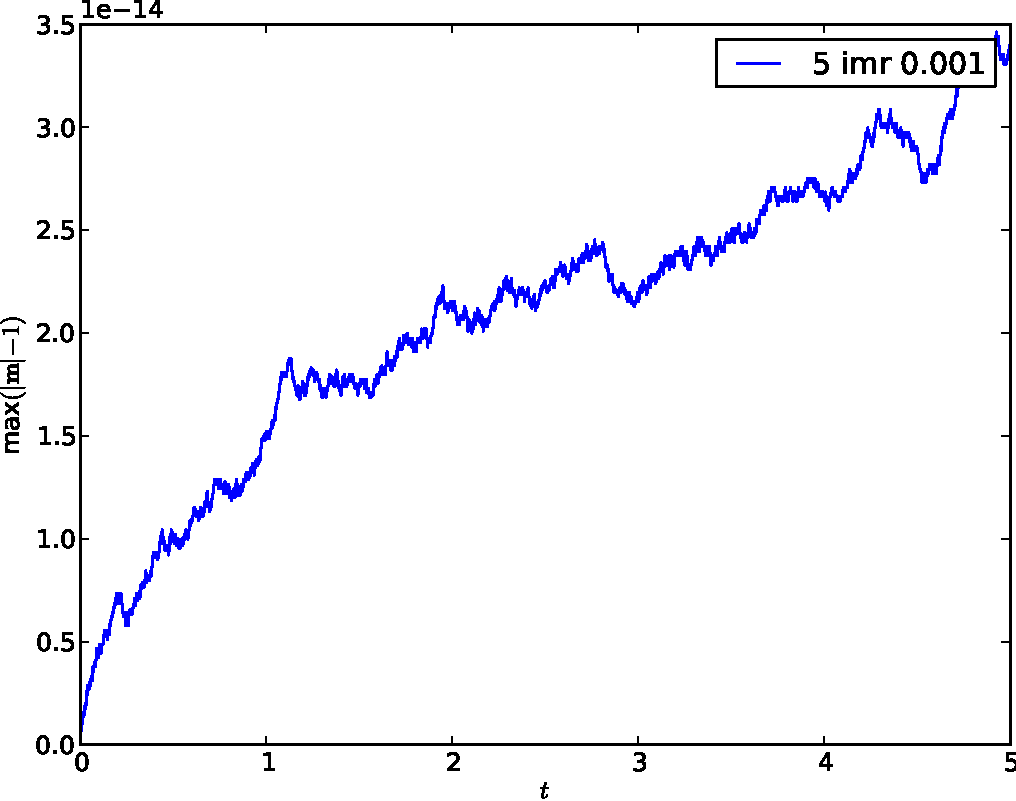
\includegraphics[width=0.8\textwidth]{plots/2d_wave_solution_m_length/lnodal-maxmathbfm-1vst.pdf}
  \caption{Evolution of the maximum error of nodal magnetisation lengths in the 2D wave example with the nodal quadrature scheme introduced above.}
  \label{fig:mean-ml-error-2d-nodal}
\end{figure}

To check that the conservation is independent of problem parameters we ran a parameter sweep using: square and triangle elements; 36, 441 and 6561 nodes; time steps of $0.1$, $0.01$ and $0.001$; and damping parameters of $1$, $0.1$, $0.001$ and $0$.
The maximum length error over all parameter sets, all time steps and all nodes when using nodal quadrature was 2.364775e-12, when using Gaussian quadrature it was 0.013746647.
This clearly demonstrates the necessity and effectiveness of the nodal quadrature scheme for retaining the conservation properties of the implicit midpoint rule.
% using the same data as for the figures above, look in their folders for parameter sets data parsing command: parse.py -d /mnt/moredata/optoomph/user_drivers/micromagnetics/experiments/parameter_sweeps/parameter_file_0/ -l=-dt -l=-damping --split=-integration --print-data max-max-ml --print-data ml -l=initial_nnode


??ds describe very long time behaviour in \autoref{fig:mean-ml-error-2d-nodal-long-time}.

\begin{figure}[ht!]
  \centering
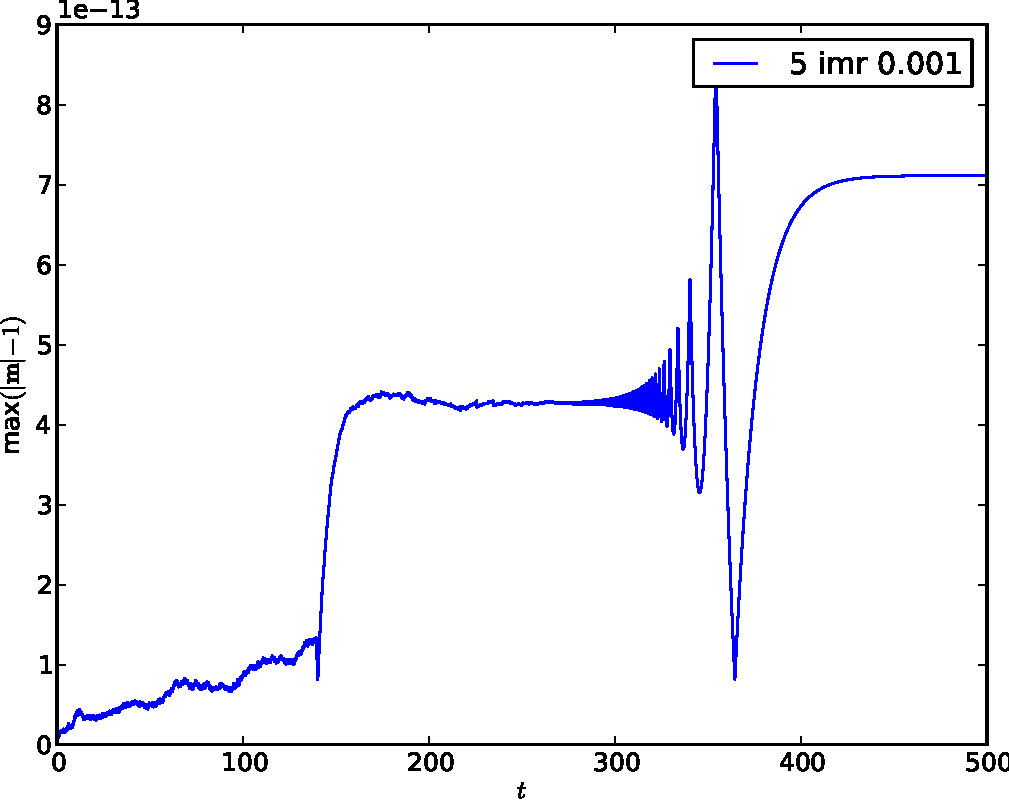
\includegraphics[width=0.8\textwidth]{plots/2d_wave_solution_m_length_long_time/-maxmathbfm-1vst.pdf}
\caption{Evolution of the maximum error of nodal magnetisation lengths in the 2D wave example with the nodal quadrature scheme over a very long time period.}
\label{fig:mean-ml-error-2d-nodal-long-time}
\end{figure}



\subsection{Effect of Newton tolerance}
\label{sec:effect-newt-toler-m-conservation}

Since the non-linear residual \eqref{eq:weak-llg} used in the derivation of the conservation properties is only true up to the accuracy of the linearisation method we would expect to see some effect when modifying this accuracy.
In our model Newton's method is used for linearisation (see \autoref{sec:newt-meth}) so the relevant measure of accuracy is the Newton tolerance.

The obvious experiment to carry out would be to vary the Newton tolerance and examine how the error in $\abs{\mv}$ is affected.
However Newton's method extremely quickly meaning that the final residual is sometimes orders of magnitude smaller than the tolerance, this would hide any corrolation between the tolerance and the error.
Instead we plot the error against the actual maximum residual obtained (specifically: the mean over time steps of $\norm{\rv}_\infty$ after the Newton method has converged). 
The results are shown in \autoref{fig:mean-ml-error-2d-nodal-newton-tests}, there is a clear corrolation between small residuals and small length errors.


\begin{figure}[ht!]
  \centering
  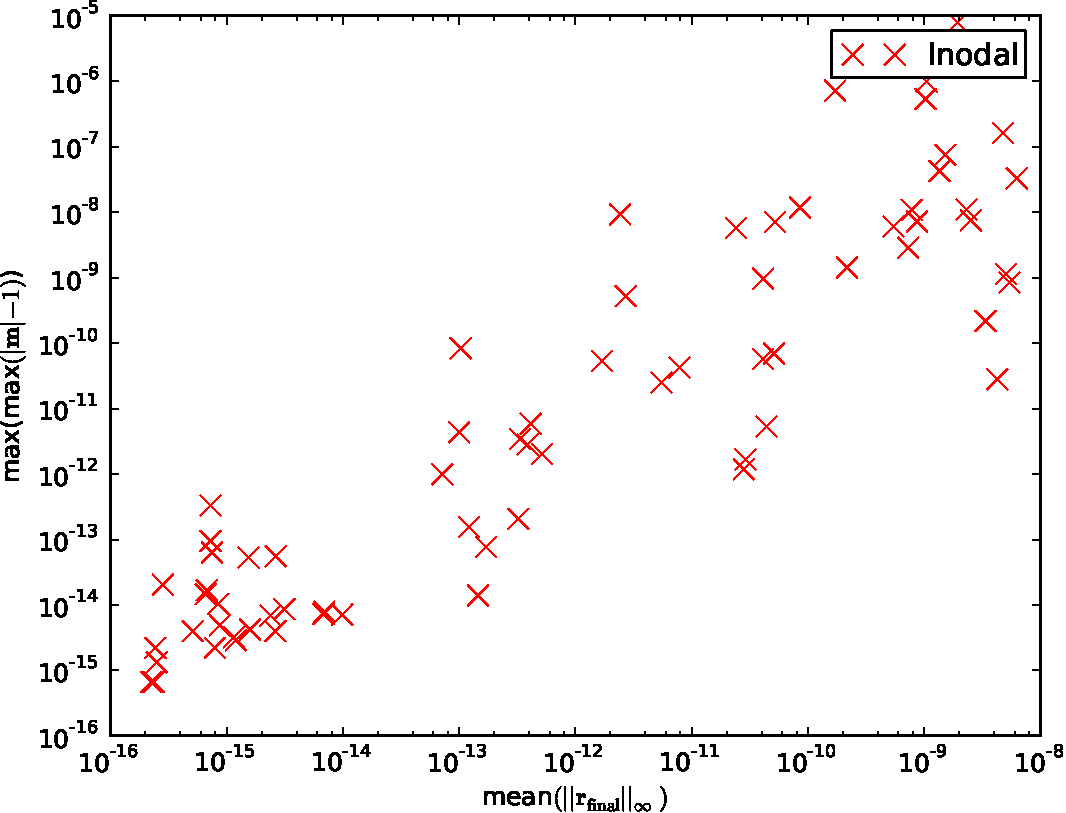
\includegraphics[width=0.8\textwidth]
  {plots/2d_wave_solution_m_length_newton_res/-maxmaxmathbfm-1vsmeanmathbfr_mathrmfinal_infty.pdf}
  \caption{Corrolation between maximum error of nodal magnetisation lengths and largest maximum Newton residual after convergence in the 2D wave example with the nodal quadrature scheme over a very long time period.}
  \label{fig:mean-ml-error-2d-nodal-newton-tests}
\end{figure}


\subsubsection{Adaptivity}

It remains to demonstrate that the adaptivity scheme introduced in \autoref{sec:adaptive-imr} is effective for the finite element problem with nodal integration.
Since there is still no relationship with previous time step sizes in the conservation proofs with nodal integration we don't expect there to be any issues with variable step size and conservation.

Additionally our discretisation can be written as semi-discretisation in space (giving a system of ODEs) followed by the application of IMR in time.
Hence we have no reason to expect the adaptive IMR to behave any differently to in the pure ODE case.






%%% Local Variables:
%%% mode: latex
%%% TeX-master: "main"
%%% End:
